\documentclass{article}
\usepackage{titlesec}
\usepackage{mathtools, amsmath, amssymb}
\usepackage{algorithm, algorithmic}
\usepackage{tikz}
\usetikzlibrary{positioning,arrows, shapes}
\newcommand{\sectionbreak}{\clearpage}
\newcommand{\xor}{\oplus}
\newcommand{\N}{\mathbb{N}}

\tikzstyle{people}=[draw, fill=green!30, minimum size = 4em]
\tikzstyle{message}=[draw, minimum size=5em, execute at begin node=\setlength{\baselineskip}{0pt}\tiny]
\tikzstyle{key}=[draw, fill=red!25, execute at begin node=\setlength{\baselineskip}{0pt}\tiny]
\tikzstyle{enc} = [fill=blue!10, regular polygon, regular polygon sides=3,shape border rotate = 180]
\tikzstyle{dec}=[fill=blue!10, regular polygon, regular polygon sides=3]

\author{Matteo Secco}
\title{Computer Security}


\begin{document}
\maketitle
\newpage
\tableofcontents
\newpage

\section{Introduction to Computer Security}
\subsection{Security requirements}
\paragraph{CIA Paradighm}
\begin{description}
\item[Confidentiality] Information can be accessed only by authorized entities
\item[Integrity] information can be modified only by authorized entities, and only how they're entitled to do
\item[Availability] information must be available to entitled entities, within specified time constraints
\end{description}
The engineering problem is that \textbf{A} conflicts with \textbf{C} and \textbf{I}

\section{Computer Security Concepts}
\subsection{General concepts}

\paragraph{Vulnerability} Something that allows to violate some CIA constraints
\begin{itemize}
\item The physical behaviour of pins in a lock
\item A software vulnerable to SQL injecton
\end{itemize}

\paragraph{Exploit} A specific way to use one or more vulnerability to violate the constraints
\begin{itemize}
\item lockpicking
\item the strings to use for SQL injection
\end{itemize}

\paragraph{Assets} what is valuable/needs to be protected
\begin{itemize}
\item hardware
\item software
\item data
\item reputation
\end{itemize}

\paragraph{Thread} potential violation of the CIA
\begin{itemize}
\item DoS
\item data break
\end{itemize}

\paragraph{Attack} an \underline{intentional} use of one or more exploits aiming to compromise the CIA
\begin{itemize}
\item Picking a lock to enter a building
\item Sending a string creafted for SQL injection
\end{itemize}

\paragraph{Thread agent} whoever/whatever may cause an attack to occour
\begin{itemize}
\item a thief
\item an hacker
\item malicious software
\end{itemize}

\paragraph{Hackers, attackers, and so on}
\begin{description}
\item[Hacker] Someone proficient in computers and networks
\item[Black hat] Malicious hacker
\item[White hat] Security professional
\end{description}

\paragraph{Risk} statistical and economical evaluation of the exposure to damage because of vulneravilities and threads\\
$Risk = \underbrace{Assets \times Vulnerabilities}_\text{controllable} \times \underbrace{Threads}_\text{independent}$
\paragraph{Security} balance of (vulnerability reduction+damage containment) vs cost

\subsection{Security vs Cost} 

\paragraph{Direct cost}
\begin{itemize}
\item Management
\item Operational
\item Equipment
\end{itemize}

\paragraph{Indirect cost}
\begin{itemize}
\item Less usability
\item Less performance
\item Less privacy
\end{itemize}

\paragraph{Trust} We must \textbf{assume} something as secure
\begin{itemize}
\item the installed software?
\item our code?
\item the compiler?
\item the OS?
\item the hardware?
\end{itemize}


\section{Introduction to crypthography}
\paragraph{Kerchoffs' Principle} The security of a (good) cryptosystem relies only on the security of the key, never on the secrecy of the algorithm
\subsection{Perfect Chipher}
\begin{itemize}
\item $P(M=m)$ probability of observing message m
\item $P(M=m|C=c)$ probability that the message was m given the observed cyphertext c
\end{itemize}
\paragraph{Perfect cypher: } $P(M=m|C=c)=P(M=m)$
\paragraph{Shannon's theorem} in a perfect cipher $|K|\geq |M|$
\paragraph{One Time Pad} a real example of perfect chipher
\begin{algorithm}
\caption{One Time Pad}
\begin{algorithmic}
\REQUIRE $len(m)=len(k)$
\REQUIRE keys not to be reused
\RETURN $k \xor m$
\end{algorithmic}
\end{algorithm} 

\paragraph{Brute Force} perfect chyphers are immune to brute force (as many "reasonable" messages will be produced). Real world chiphers are not.\\
A real chipher is vulnerable if there is a way to break it that is faster then brute forcing

\paragraph{Types of attack}
\begin{description}
\item[Ciphertext attack] analyst has only the chipheertexts
\item[Known plaintext attack] analyst has some pairs of plaintext-chiphertext
\item[Chosen plaintext attack] analyst can choose plaintexts and obtain their respective ciphertext
\end{description}

\subsection{Symmetric encryption}
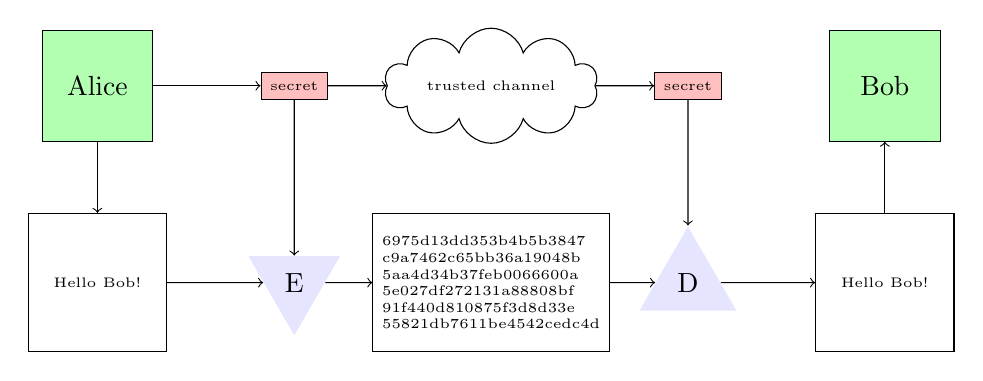
\begin{tikzpicture}[node distance=2.5cm,auto]
	\node[people] (alice) {Alice};
	\node[message, below of=alice] (msgAlice) {Hello Bob!};
	\node[enc, right of=msgAlice](e){E};
	\node[key, above of=e] (keyAlice) {secret};
	\node[message, right of=e, align=left] (chip) {
		6975d13dd353b4b5b3847\\
		c9a7462c65bb36a19048b\\
		5aa4d34b37feb0066600a\\
		5e027df272131a88808bf\\
		91f440d810875f3d8d33e\\
		55821db7611be4542cedc4d};
	\node[cloud, draw, right of = keyAlice, aspect=3] (chan) {\tiny trusted channel};
	\node[dec, right of=chip](d){D};
	\node[key, above of=d](keyBob){secret};
	\node[message, right of=d](msgBob){Hello Bob!};
	\node[people, above of=msgBob](bob){Bob};
	\path[->] (alice) edge (msgAlice);
	\path[->] (msgAlice) edge (e);
	\path[->] (alice) edge (keyAlice);
	\path[->] (keyAlice) edge (e);
	\path[->] (keyAlice) edge (chan);
	\path[->] (chan) edge (keyBob);
	\path[->] (e) edge (chip);
	\path[->] (chip) edge (d);
	\path[->] (keyBob) edge (d);
	\path[->] (d) edge (msgBob);
	\path[->] (msgBob) edge (bob);
\end{tikzpicture}

Use \textbf{K} to both encrypt and decript the message\\
Scalability issue\\
Key agreement issue

\subsubsection{Ingredients} 
\begin{description}
\item[Substitution] Replace each byte with another (ex: caesar chipher)
\item[Transposition] swap the values of given bits (ex: read vertically)
\end{description}

\subsection{Asymetric encryption}
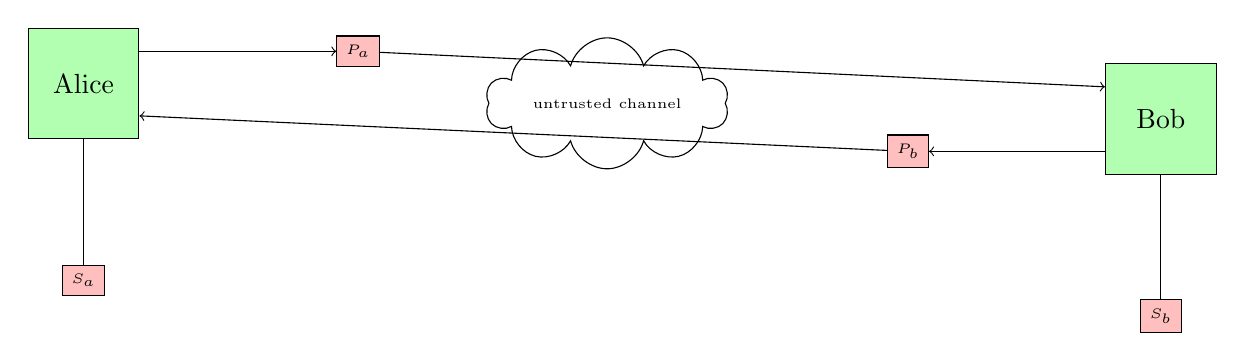
\begin{tikzpicture}[node distance=2.5cm];
	\node[people] (alice) {Alice};
	\node[key, right=of alice.30] (pubAlice) {$P_a$};
	\node[cloud, aspect=3, right of=pubAlice, draw, anchor=45+90] (chan) {\tiny untrusted channel};
	\node[key, right= of chan.330] (pubBob) {$P_b$};
	\node[people, right of = pubBob, anchor=210] (bob) {Bob};
	\node[key, below of=alice] (secAlice) {$S_a$};
	\node[key, below of=bob] (secBob) {$S_b$};
	\path[->] (alice.30) edge (pubAlice);
	\path[->] (pubAlice) edge (bob.150);
	\path[->] (bob.210) edge (pubBob);
	\path[->] (pubBob) edge (alice.-30);
	\path[-] (alice) edge (secAlice);
	\path[-] (bob) edge (secBob);
\end{tikzpicture}
Each user owns a private and a public key ($S_i,P_i$), where the public key is publicly available. The cryptoalgorithm is designed so that messages encrypted using $P_i$ can only be decrypted using $S_i$. This allows Alice to encrypt a message using $P_{bob}$, and Bob (and nobody else) to decrypt is using $S_{bob}$.
Also, to prove its identity, Bob could send a message encrypted using $P_{bob}$. When Alice manages to decrypt is using $P_{bob}$, she can be sure that the message came from Bob


\subsection{Hash functions}
A function $H: X \to Y$ having $|X|=\infty$ but $|Y|=k \in \mathbb{N}$. This means $|Y|<|X|$, leading to \underline{collisions}: couples $x_1,x_2\in X: H(x_1)=H(x_2)$.
\paragraph{Safery properties} are proberties needed to ensure robustness of $H$. In particular, it must be computationally infeasible to find:
\begin{description}
\item[preimage attack resistance] $x: H(x)=h$ with $h$ known/crafted
\item[second preimage attack resistance] $y: y \neq x \wedge H(x)=H(y)$, where $x$ is known/crafted
\item[collision resistance] $x, y: H(x)=H(y)$  
\end{description}

\end{document}